\documentclass[11pt,a4paper]{article}
\usepackage[utf8]{inputenc}
\usepackage[T1]{fontenc}
\usepackage{amsmath,amsfonts,amssymb}
\usepackage{apacite}
\usepackage{natbib}
\usepackage{graphicx}
\usepackage{booktabs}
\usepackage{threeparttable}
\usepackage{url}
\usepackage{hyperref}
\usepackage[margin=2.5cm]{geometry}
\usepackage{setspace}
\onehalfspacing

\newcommand{\Var}{\text{Var}}
\newcommand{\Cov}{\text{Cov}}

% Define \sym command for significance stars from esttab
\newcommand{\sym}[1]{{#1}}

\title{Estimating the Value of CEOs in Privately Held Businesses\thanks{Project no. 144193 has been implemented with the support provided by the Ministry of Culture and Innovation of Hungary from the National Research, Development and Innovation Fund, financed under the KKP\_22 funding scheme. This project was funded by the European Research Council (ERC Advanced Grant agreement number 101097789). The views expressed in this research are those of the authors and do not necessarily reflect the official view of the European Union or the European Research Council. \emph{Author contributions:} Conceptualization and study design: Koren, Orbán and Telegdy. Data curation, integration and quality assurance: Szilágyi and Vereckei. Statistical analysis: Koren and Telegdy. Writing the original draft: Koren. Review and editing: Koren, Orbán, Szilágyi, Telegdy and Vereckei. \emph{AI disclosure:} Claude Sonnet 4 was used to write and edit the research code and to format the manuscript (such as editing tables, figures, references, creating summaries). All code and text generated by AI tools were reviewed and edited by the authors. All authors have read and agreed to the published version of the manuscript. \emph{Data availability statement:} The data underlying this article cannot be shared publicly due to privacy and licensing restrictions. The replication package is available at \url{https://github.com/korenmiklos/ceo-value}.}}

\author{Miklós Koren\thanks{Central European University, HUN-REN Centre for Economic and Regional Studies, CEPR and CESifo. E-mail: korenm@ceu.edu} \\
        Krisztina Orbán\thanks{Monash University.} \\
        Bálint Szilágyi\thanks{HUN-REN Centre for Economic and Regional Studies.} \\
        Álmos Telegdy\thanks{Corvinus University of Budapest.} \\
        András Vereckei\thanks{HUN-REN Centre for Economic and Regional Studies, Institute of Economics.}}

\date{\today}

\begin{document}

\maketitle

\begin{abstract}
We develop a model-based approach to measure CEO value in privately held businesses, holding fixed inputs chosen by owners while substituting out variable inputs optimized by managers. Using the universe of Hungarian firms and their CEO networks over three decades (1992-2022), we estimate skill differences that translate into measurable productivity impacts. Most importantly, we develop a novel placebo-controlled event study design that reveals 78 percent of typical fixed-effect estimates reflect noise rather than true CEO effects. The naive comparison shows firms hiring better CEOs outperform those hiring worse CEOs by 25.3 percent, but placebo transitions---randomly assigned fake CEO changes excluding actual transition periods---generate a 19.7 percent spurious effect. The true causal impact is thus 5.5 percent: statistically significant and economically meaningful, but only 22 percent of the raw correlation. This methodology addresses a fundamental identification challenge in the managerial effects literature and suggests new approaches for using CEO quality measures in empirical work.
\end{abstract}

\textbf{Keywords:} CEO value, private firms, productivity

\textbf{JEL Classification:} [To be added]

\newpage

\section{Introduction}

How much do CEOs matter for firm performance? The answer has profound implications for corporate governance, executive compensation, and economic policy, yet measuring CEO value remains one of the most challenging problems in empirical economics. While a large literature documents substantial manager effects---\citet{Bertrand2003-io} find that switching from a 25th- to 75th-percentile CEO alters return on assets by 4 percentage points in U.S. public firms, and \citet{metcalfe2023managers} attribute 20-30 percent of store-level sales variance to managers---these estimates may substantially overstate true CEO importance.

The fundamental challenge is separating genuine managerial skill from spurious correlations. The econometric literature has long recognized this problem: \citet{gaure2014correlation} demonstrates correlation bias in two-way fixed effects models, \citet{bonhomme2023much} show that limited mobility bias severely contaminates firm and worker effect estimates, and \citet{andrews2008high} find that accounting for such biases reduces coefficients by 50 percent or more. These theoretical concerns suggest we may be dramatically overstating individual managers' importance.

This measurement problem is particularly acute for privately held businesses, which constitute the vast majority of economic activity worldwide yet remain understudied due to data limitations. While public companies provide stock returns and detailed compensation data, private firms offer neither, requiring new approaches to value measurement. Moreover, existing studies typically examine hundreds or thousands of firms, limiting statistical power to separate signal from noise in manager effects.

Against this backdrop, quasi-experimental evidence provides sobering benchmarks. \citet{bennedsen2020ceos} exploit CEO hospitalizations as exogenous shocks in Danish firms, finding that permanent CEO absence would reduce returns by roughly 7 percent---substantial, but far smaller than correlational estimates suggest. Similarly, \citet{chandra2016health} find hospital manager effects explain only 5 percent of risk-adjusted mortality variance after accounting for patient selection. These causal estimates hint that true CEO effects, while meaningful, are much smaller than standard methods imply.

This paper addresses these challenges by developing a novel methodology to measure CEO value in privately held businesses and applying it to the universe of Hungarian firms over three decades. Our approach reveals a startling finding: approximately 77 percent of what standard methods identify as CEO effects are spurious. The true causal impact of CEO quality on firm performance is 5.5 percent---economically meaningful but only one-fifth of the raw correlation.

We make four main contributions:

\textbf{First}, we develop a placebo-controlled event study methodology that separates true CEO effects from spurious correlations. By constructing placebo CEO transitions---randomly assigned fake changes that exclude actual transition periods---we isolate mechanical biases from genuine impacts. The naive comparison shows firms hiring better CEOs outperform those hiring worse CEOs by 25.3 percent. Remarkably, placebo transitions generate a 19.7 percent effect despite no actual management change. The true causal impact is thus 5.5 percent: the difference between actual and placebo effects.

\textbf{Second}, we ground this empirical strategy in a model-based framework that clarifies what we can and cannot measure. Building on \citet{Lucas1978-rp} and decreasing returns models of \citet{AtkesonKehoe2005JPE, McGrattan2012RED}, we explicitly separate owner-controlled inputs (capital, organizational structure) from manager-controlled inputs (labor, materials). This distinction is crucial: CEOs receive credit for many factors outside their control. Our framework identifies the marginal contribution of CEO skills to firm surplus while holding fixed the inputs chosen by owners.

\textbf{Third}, we implement this approach using extraordinary data: the universe of Hungarian firms over three decades (1992-2022). We track 1,063,172 firms and 1,030,470 unique CEOs, identifying a connected network of 189,108 managers who lead multiple firms. This scale dwarfs previous studies---\citet{fee2013managers} examine 500 firms, \citet{fenizia2022managers} study 433 public administrations, even \citet{metcalfe2023managers} cover 66,000 stores. Our data enables precise estimation of manager effects through 51,736 firms with exactly one CEO change, providing statistical power to separate signal from noise that smaller samples cannot achieve.

\textbf{Fourth}, we provide practical guidance for future research using manager quality measures. Given that 77 percent of apparent CEO effects reflect noise, researchers should: (i) incorporate observable manager characteristics to reduce measurement error; (ii) place CEO quality measures on the left-hand side of regressions where noise is less problematic; (iii) never use them as right-hand side variables where attenuation bias dominates; (iv) avoid simple correlations where inflated variance misleads. These guidelines have immediate implications for the large literature using manager fixed effects.

Our findings reconcile the seemingly contradictory evidence on CEO importance. The true causal effect of 5.5 percent aligns remarkably with quasi-experimental studies, confirming that CEOs matter but far less than correlational estimates suggest. This has profound implications: policies targeting managerial quality will have more modest impacts than raw correlations imply, executive compensation debates rest on inflated effect sizes, and much of the variation in firm performance attributed to leadership reflects other factors. By providing a methodology to separate signal from noise in manager effects, we enable more rigorous analysis of when, how, and how much management matters for economic outcomes.


\section{Modeling Framework}
Firms produce output using a Cobb-Douglas production function that incorporates both fixed and variable inputs. Owing to the presence of fixed inputs, technology exhibits decreasing returns to scale. This will pin down the scale of the firm even when markets are perfectly competitive and the firm is a price taker in both input and output markets \citep{AtkesonKehoe2005JPE,McGrattan2012RED}.\footnote{Alternatively, we could assume that firms face downward sloping residual demand curves, which would make the \emph{revenue production function} decreasing returns to scale. As long as residual demand is isoelastic, the analytical derivation of the model remains unchanged. The only difference is that the parameters have a different interpretation: the revenue elasticity of an input is the product of the input's share in revenue and $1-1/\sigma$, where $\sigma$ is the elasticity of residual demand \citep{DeLoecker2011Econometrica}.}

The production function for firm $i$ with manager $m$ at time $t$ is:
\begin{equation}\label{eq:production}
Q_{imt} = \Omega_{it}A_i Z_{m}  K_{it}^\alpha L_{imt}^{\beta} M_{imt}^{\gamma}
\end{equation}
where $\Omega_{it}$ is residual total factor productivity, $A_i$ represents time-invariant organizational capital and immaterial assets (location, brand value), $Z_m$ captures manager skill, $K_{it}$ is physical capital, $L_{imt}$ is labor input, $M_{imt}$ is intermediate input usage. The parameters $\alpha$, $\beta$ and $\gamma$ represent the elasticities with respect to physical capital, labor and material inputs, respectively. We denote $\chi := 1 - \beta - \gamma$. Conditional on productivity, organizational capital and manager skill, the production function exhibits decreasing returns to scale, $\alpha + \beta + \gamma < 1$. In a traditional production function with only capital, labor and material as inputs, $\Omega$, $A$ and $Z$ would all be lumped together as \emph{total factor productivity}.

We assume managers optimize variable inputs $L_{imt}$ and $M_{imt}$ while taking fixed inputs $A_{i}$ and $Z_m$ and physical capital $K_{it}$ as given. In private businesses, owners typically have direct control over fixed inputs, including large-scale investments in organizational and physical capital \citep{Navaretti2010EFIGE}. Managers, on the other hand, are responsible for day-to-day operations and variable input choices.

Output is sold at sector-specific price $P_{st}$, making the revenue of the firm $R_{imst} = P_{st}Q_{imt}$. The firm faces a wage rate $W_{st}$ for labor input, price $\varrho_{st}$ for intermediate inputs. After straightforward algebra solving for the optimal labor and intermediate input choices, the firm's revenue can be expressed as:
\begin{equation}\label{eq:revenue}
R_{imst} = (P_{st}\Omega_{it}A_i Z_m)^{1/\chi}
K_{it}^{\alpha/\chi}
W_{st}^{-\beta/\chi}
\varrho_{st}^{-\gamma/\chi}
(1-\chi)^{(1-\chi)/\chi}.
\end{equation}
Revenue is increasing in fixed inputs $A_i$ and $Z_m$, physical capital $K_{it}$, and decreasing in the wage rate $W_{st}$ and material input price $\varrho_{st}$. Higher prices $P_{st}$ and productivity $\Omega_{it}$ also increase revenue. Note that because $\chi<1$, the elasticity of revenue with respect to fixed inputs is greater than the elasticity in the production function, i.e. $\alpha/\chi > \alpha$. This is because the firm can leverage its fixed inputs to increase revenue more than proportionally by hiring more variable inputs.

As is usual under Cobb-Douglas production functions, the share of revenue accruing to each input is constant over time and across firms, equal to their elasticity in the production function. We define the rent accruing to fixed factors (including physical capital) 
\begin{equation}\label{eq:rent}
S_{imst} = R_{imst} - W_{st}L_{imt} - \varrho_{st}M_{imt} = \chi R_{imst}.
\end{equation}
Taking logarithms of equations \eqref{eq:revenue} and \eqref{eq:rent}, we can express the log surplus as:      
\begin{equation}\label{eq:log_surplus}
s_{imst} = C+\frac\alpha\chi k_{it} + \frac1\chi {z}_{m} + \frac1\chi p_{st} + \frac1\chi{\omega}_{it}+\frac1\chi a_i 
- \frac\beta\chi w_{st} - \frac\gamma\chi \rho_{st},
\end{equation}
where $C$ is a constant only depending on fixed parameters, $k_{it} = \ln K_{it}$, ${z}_{m} = \ln Z_m$ , $ p_{st} = \ln P_{st}$, ${\omega}_{it} = \ln\Omega_{it}$, $a_i = \ln A_i$, and $w_{st} = \ln W_{st}$, $\rho_{st} = \ln \varrho_{st}$. 

Equation \eqref{eq:log_surplus} shows how surplus depends on manager skills, holding fixed the inputs chosen by the owner and the input and output prices prevailing in the sector. Taking two managers $m$ and $m'$ with skills ${z}_m$ and ${z}_{m'}$ at the same firm, the change in surplus attributable to the new manager is:
\begin{equation}\label{eq:manager_change}
s_{im'st} - s_{imst} = \frac1\chi({z}_{m'} - {z}_{m}).
\end{equation}
The \emph{value} of the new manager to the owners of the firm is the change in surplus. This value is proportional to the difference in manager skills, scaled by the inverse of the elasticity of revenue with respect to fixed inputs $\chi$. In what follows, we aim to measure this value by estimating the change in surplus following a manager change.

\paragraph{Estimable equation.} In absence of observing organization capital and input prices, we can substitute these out with fixed effects, leading to the following estimable equation:
\begin{equation}\label{eq:estimation}
s_{imst} = \frac\alpha\chi k_{it}  + \frac1\chi\tilde{z}_m + \lambda_i + \mu_{st} + \tilde \omega_{it}
\end{equation}
where $\lambda_i = a_i/\chi$ is a firm fixed effect capturing time-invariant organizational capital, $\mu_{st} = C + p_{st}/\chi - \beta w_{st}/\chi - \gamma\rho_{st}/\chi$ is an industry-time fixed effect capturing sector-specific prices and wages, and $\tilde\omega_{it} = \omega_{it}/\chi$ is a rescaled time-varying firm productivity shock. 

Assuming that residual productivity $\tilde\omega_{it}$ is uncorrelated with manager skills and physical capital, we can estimate the model using ordinary least squares with fixed effects (OLSFE). Note that we do \emph{not} assume that manager skills are uncorrelated with physical capital, organizational capital or sectoral prices. It may well be the case that better firms with good price conditions hire better managers and invest more. 

Given our estimated parameters and fixed effects, we can recover manager skills as:
\begin{equation}\label{eq:estimated}
\hat z_m :=
\frac1{N_m}\sum_{i,s,t}(
        \hat\chi s_{imst} -  \hat\alpha k_{it}  -\hat\chi \lambda_i -\hat\chi \mu_{st}
). 
\end{equation}
We remove the contribution of physical capital, firm and industry-year fixed effects from log surplus to obtain a \emph{residualized surplus} $\tilde s_{imst}$. Because $\omega_{it}$ is assumed to be mean zero independent of $m$, we can estimate $\hat z_m$ as the average of $\tilde s_{imst}$ across all observations for manager $m$. This gives us a consistent estimate of manager skill when $N_m$ is large, but includes average residual productivity $\hat\omega_{it}$.\footnote{This is equivalent to including a manager fixed effect in the regression, similar in spirit to \citet{Abowd1999Econometrica} and \citet{Card2018JoLE}. This notation emphasizes that manager effects estimated from fewer observations are noisier.}

Because this estimate of manager effects is noisy when $N_m$ is small, we implement a placebo strategy to estimate the true effects of managers, as described in ??.

\section{Data and Measurement}
\paragraph{Main data sources.} Our analysis uses comprehensive administrative data on Hungarian firms between 1992 and 2022, created by merging balance sheet and financial statement data with firm registry information. The balance sheet data comes from \citet{merleg2024} and contains financial information for essentially all Hungarian firms required to file annual reports. The firm registry data comes from \citet{cegjegyzek2024} and includes information on firm registration, ownership structure, and director appointments.\footnote{The data cannot be publicly shared due to privacy and licensing restrictions. The replication package available at https://github.com/korenmiklos/ceo-value describes how to get access to the data.}

The balance sheet dataset contains detailed financial information including sales revenue, export revenue, employment, tangible and intangible assets, raw material and intermediate input costs, personnel expenses, and ownership indicators for state and foreign control.

Registry information is collected by the Hungarian Corporate Court, which maintains legally mandated public records on firms \citep{cegtv}. These records include information on company representatives---individuals authorized to act on behalf of the firm in legal and business matters. Representatives may include CEOs and other executives, but also lower-level employees with signatory rights. We exclude the rare instances where the representative is a legal entity. The dataset is structured as a temporal database: each entry has an effective date interval and reflects the state of representation at a given time. Updates occur not only when positions change but also when personal identifiers (e.g., address) are modified or when reporting standards evolve. Start and end dates are often missing, and prior to 2010, the data does not contain unique numerical identifiers for individuals.

We resolve individual identities by linking records based on name, date of birth, mother's name, and home address, creating a unique identifier for each person. This entity resolution step enables tracking of representatives over time and across firms. To construct an annual panel of top managers, we infer the period of service for each representative using available date bounds and sequential information. A representative is considered active in a given year if their tenure includes June 21 of each year.

Because job titles are not standardized, identifying the CEO requires heuristic rules. When an explicit title such as \emph{managing director} is available, we classify the individual accordingly. For firms lacking such labels, we assume that all representatives are CEOs if the number of representatives is three or fewer. If there are more than three and one of them was previously identified as a CEO, we assign the CEO role based on continuity. This approach allows us to systematically identify the firm's top executive across years.

\paragraph{Target population.} Our initial sample contains 1,063,172 firms spanning 31 years with 10,151,997 firm-year observations. Table \ref{tab:sample} shows the temporal distribution of observations in our final sample. The sample exhibits steady growth from 61,730 firms in 1992 to 390,632 firms in 2022. This expansion reflects the growth of entrepreneurship in Hungary following the transition to a market economy.

\begin{table}[htbp]
\centering
\caption{Sample Over Time}
\label{tab:sample}
\begin{tabular}{*{6}{c}}
\toprule
Year & \shortstack{Total\\firms} & \shortstack{Sample\\firms} & CEOs & \multicolumn{2}{c}{Connected component} \\
\cmidrule(lr){5-6}
 & & & & Firms & CEOs \\
\midrule
1992 &       98,780 &       25,833 &       31,746 &        1,423 &        1,713 \\
1995 &      171,759 &       45,828 &       53,704 &        2,659 &        3,028 \\
2000 &      280,386 &       73,837 &       83,862 &        4,783 &        5,100 \\
2005 &      326,905 &       92,242 &      104,380 &        6,283 &        6,474 \\
2010 &      384,570 &      103,892 &      116,680 &        7,405 &        7,084 \\
2015 &      433,371 &      116,543 &      124,960 &        8,332 &        7,488 \\
2020 &      424,501 &      115,755 &      123,504 &        7,789 &        6,841 \\
2022 &      454,106 &      113,387 &      121,730 &        7,419 &        6,509 \\
\midrule
Total &    1,063,172 &      217,737 &      339,993 &       14,416 &       22,001 \\
\bottomrule
\end{tabular}
\begin{minipage}{12cm}
\footnotesize
\textit{Notes:} This table presents the evolution of the sample from 1992 to 2022. Column (1) shows the total number of distinct firms with balance sheet data. Column (2) shows the number of distinct firms after applying data quality filters. Column (3) shows the number of distinct CEOs. Columns (4) and (5) show the subset of distinct firms and CEOs that belong to the largest connected component of the manager network, where managers are connected if they have worked at the same firm. The table shows every fifth year plus the first year (1992), last year (2022), and totals of distinct counts. \end{minipage}
\end{table}


Some firms have more than one CEO at a time. Among the 12,726,597 firm-year observations with CEO information, the vast majority (82\%) have a single CEO. However, 15\% of firm-years have two CEOs, 2\% have three CEOs, and small fractions have even larger numbers of CEOs (Table \ref{tab:ceo_patterns}, Panel A). Over the life of a firm, it is not uncommon for multiple individuals to hold the CEO title, reflecting changes in leadership and organizational structure. As the second column of the Table shows, however, a large fraction of firms (63\%) is managed by the same CEO during their entire lifetime.

\begin{table}[htbp]
\centering
\caption{Number and Job Spell of CEOs}
\label{tab:ceo_patterns}
\begin{minipage}{0.48\textwidth}
\centering
\textbf{Panel A: Number of CEOs}
\begin{tabular}{lcc}
\toprule
CEOs & Firm-Year & Firm \\
\midrule
1 & 79\% & 79\% \\
2 & 18\% & 17\% \\
3 & 3\% & 3\% \\
4+ & 1\% & 1\% \\
Total &    1,884,566 &      402,875 \\
\bottomrule
\end{tabular}

\end{minipage}
\hfill
\begin{minipage}{0.48\textwidth}
\centering
\textbf{Panel B: Spell Lengths}
\begin{tabular}{lcc}
\toprule
Length & Actual & Placebo \\
(Years) & Spells & Spells \\
\midrule
1 & 22\% & 27\% \\
2 & 15\% & 19\% \\
3 & 11\% & 14\% \\
4+ & 51\% & 40\% \\
Total &      107,957 &       14,978 \\
\bottomrule
\end{tabular}

\end{minipage}
\begin{tablenotes}[flushleft]
\footnotesize
\item\textbf{Panel A} reports the distribution of CEOs at firms. Column 1 shows the percentage of firm-year observations with 1, 2, 3, or 4+ CEOs. Column 2 shows the percentage of firms with 1, 2, 3, or 4+ CEO spells over the sample period. \textbf{Panel B} reports the distribution of CEO spell lengths. A CEO spell is defined as a continuous period of the same person serving at the same firm.
Actual spells are computed from the administrative data (1992-2022), excluding firms with more than one CEO per year and the last spell (because these end in firm death, not CEO change). Placebo spells follow an exponential distribution with the same exit probability as actual CEOs. We exclude firms where a placebo spell would overlap with an actual spell.
\end{tablenotes}
\end{table}

Panel B of Table \ref{tab:ceo_patterns} shows the distribution of CEO spell lengths. We exclude the last CEO of the firm (and hence all firms with only a single CEO), because these spells end in firm death or sample truncation, not CEO turnover. The typical CEO is replaced with a hazard rate of about 20\%/year. The empirical distribution of spell lengths is displayed in the first column, with a mode at one year (23\% of spells).

Column 2 of Panel B shows the distribution of spell lengths for placebo CEO changes, which were generated by randomly assigning CEO exit times to firms with long CEO spells. More specifically, we took firms which were lead by the same CEO in at least the first seven years of their lives. We then introduced random (``placebo'') CEO switches in these firms using the empirical hazard function of CEO change in the true data. For example, 24\% of CEOs are replaced after their first year, 22\% after their second year, and so on.\footnote{In practice, using a constant hazard rate of CEO change leads to similar results.} We then excluded the last placebo spell, to exclude sample truncation. By construction, the empirical distribution of spell lengths is very similar to that of actual CEO spells (Column 1), although small random variations are to be expected.

\paragraph{Sample definition.} 
We classify firms into broad industry using the NACE Revision 2 classification system. We exclude mining and finance, due to their different accounting, reporting and regulatory frameworks. Detailed industry-level summary statistics are presented in Table \ref{tab:industry_stats} in the Online Appendix. We also exclude firms that ever have more than two CEOs in a single year, removing 1,519,524 observations. This filter eliminates firms with potentially complex or unstable governance structures. Third, we drop firms with more than six CEO spells over the observation period, removing an additional 45,216 observations. Additionally, we exclude all firms that were ever state-owned during the observation period, as state ownership introduces different objective functions and constraints that may confound our productivity analysis of private firm management.

\paragraph{Measurement of model variables.} We measure the key variables from the theoretical framework as follows. Revenue ($R_{it}$) is the real sales revenue of the firm, inflated to 2022 prices. Capital ($K_{it}$) is measured as the book value of fixed assets (also at 2022 prices). As another variable controlled primarily by the owner, we include a dummy for whether the firm has reported any intangible assets on its balance sheet. In addition, the presence of a majority foreign owner is also measured as reported in the annual report of the firm.

We compute EBITDA (Earnings Before Interest, Taxes, Depreciation, and Amortization, $S_{it}$) as sales revenue minus personnel expenses minus material costs. Personnel expenses (wage bill inclusive of payroll taxes) and material expenditures are directly used from the financial statement. In some of the analysis, we control for firm age (years passed since foundation) and CEO tenure (years since CEO took over).

\section{Estimation}

We are interested in recovering $z_m$, the (log) skill of manager $m$. This requires estimating the production function parameters in equation \eqref{eq:estimation}, then computing the manager fixed effects using equation \eqref{eq:estimated}.

\paragraph{Production function.}
Equation \eqref{eq:estimation} controls for time-invariant firm characteristics (organizational capital, location, brand value) through firm fixed effects and sector-specific price and wage variation through industry-time fixed effects. The key identifying assumption is that residual productivity shocks $\tilde{\omega}_{it}$ are uncorrelated with manager skills and physical capital conditional on these fixed effects.

We let the production function \eqref{eq:production} and, correspondingly, surplus function \eqref{eq:estimation} vary across sectors. In addition to fixed effects, the parameters to estimate are the elasticity of output with respect to capital $\alpha$ and the share of surplus in revenue $\chi$. 

We follow \citet{Gandhi2020-nu} and use the first-order condition for the demand for variable inputs to estimate $\chi$ as one minus the share of labor and material in revenue. Hence $\chi$ is the (revenue-weighted) average of the EBITDA-revenue ratio for the industry.

Given our assumptions about fixed effects and error structure, equation \eqref{eq:estimation} can be estimated with OLSFE using \texttt{reghdfe} \citep{reghdfe}.\footnote{Structural estimates in the spirit of \citet{Olley1996-wy} yield similar results.} The resulting capital coefficient is $\alpha/\chi$, which we multiply by $\hat\chi$ to obtain the estimated capital elasticity. In addition to fixed assets, we also include a dummy for whether the firm has reported any intangible assets, and another dummy for whether it has a majority foreign owner.

To control for CEO effects when estimating the production function, we allow for firm-CEO fixed effects in \eqref{eq:estimation}. That is, instead of $z_m$ as in the model, we allow for $z_{im}$. This allows for the firm to have different TFP under different leadership, but is not yet used as a measure of CEO skill. 

There are cases when the firm has two CEOs. (More than two have been excluded from the sample.) In such cases, we repeat the observation, once for each CEO, and proceed as detailed above. This is to let these years inform the estimation of the skill of each of its CEO, as explained below.

Once we have all the parameters, we can compute the residual surplus as defined in \eqref{eq:estimated}. Because the residual surplus removes firm and industry-year fixed effects, it will always have mean zero within each firm and within each industry-year cell. To identify an interpretable manager effect, we proceed as follows.

\paragraph{Within-firm CEO changes.}
First we study the impact of within-firm CEO changes on firm surplus. If there are $n$ CEOs in a firm, we can estimate $n-1$ CEO fixed effects. We normalize the log skill of the first CEO of the firm to zero. The remaining $n-1$ CEO fixed effects are then interpreted as the difference in skills relative to the first CEO. Naturally, this calculation only makes sense for $n>1$, i.e. for firms that have at least two CEOs in the sample.

\paragraph{Largest connected component.}
We can also estimate a two-way fixed effects model for firms and managers \citep{Abowd1999Econometrica,Card2018JoLE,reghdfe} and recover the estimated manager fixed effects as measures of CEO skill. Because fixed effects are only meaningful relative to a common baseline group, we only estimate them for the largest connected component of the firm-manager network \citep{Bonhomme2023-dx}. Intuitively, the skills of two CEOs can only be compared if they ever worked for the same firm, or are connected via a path of CEOs with whom they did.

\paragraph{Event study.}
Finally, to check the dynamic effects around CEO changes, we conduct an event study analysis. This involves estimating the impact of CEO transitions on firm performance over time, allowing us to observe any pre-trends and post-trends associated with the change in leadership. 

Because we do not use any CEO observables, we compare firms hiring better CEOs against those hiring worse CEOs, as defined by their estimated fixed effects. This approach, however, suffers from potential bias because the estimated fixed effects include an average of residual TFP. Even if residual TFP is uncorrelated with CEO replacement, as we assumed, differentiating ``better'' and ``worse'' CEOs based on this noisy measure will overestimate the effect of CEO skill.

To mitigate this bias, we create a control group of firms in the same industry that did not change their CEOs during the treatment period. For these control firms, we create ``placebo'' CEO changes by randomly splitting their lifetime into CEO spells. The placebo treatment captures the bias, because it only measures the average residual TFP before and after the random splits, when CEO skill has not actually changed.  The placebo spells are constructed ensuring that the distribution of CEO tenures remains consistent with the original data.

Because our control group is also receiving a ``treatment'' (albeit a placebo), we need to use a modified version of the difference-in-differences estimator \citep{Callaway2021JoLE} that accounts for the two treatment groups \citep{Koren2023expat,Koren2024xt2treatments}. The estimated effects can be interpreted as the change in the outcome variable, relative to the baseline time period, relative to the same change in the placebo-controlled group.

UNEDITED BEGIN

Within the largest connected component, we estimate manager skills using the two-way fixed effects framework of \citet{abowd1999high}:
\begin{equation}
s_{imst} = \frac{\alpha}{\chi} k_{it} + \psi_m + \lambda_i + \mu_{st} + \varepsilon_{imst}
\end{equation}
where $\psi_m$ are manager fixed effects normalized to have mean zero across all managers in the connected component. This approach provides estimates of absolute manager skill differences that can be compared across the entire managerial labor market.

The key identifying assumption is that manager mobility is not systematically correlated with unobserved firm or time-varying productivity shocks. Recent work by \citet{metcalfe2023managers} suggests this assumption is reasonable in settings with substantial manager turnover, as in our Hungarian data.

UNEDITED END

\paragraph{Variance decomposition.} To quantify the contribution of manager skills to firm performance, we conduct a variance decomposition of various firm outcomes. Recall from equation \eqref{eq:log_surplus} that log EBITDA (and hence log revenue, up to a constant) can be written as the sum if ?? components

We first remove price effects by comparing all firms to the average firm in their industry,
\begin{equation}
s_{imst} - \Bar s_{st} = \frac1\chi a_i + \frac\alpha\chi (k_{it} - \Bar k_{st}) + \frac1\chi {z}_{m}+ \frac1\chi{\omega}_{it},
\end{equation}
where we have normalized manager and firm fixed effects to be zero in each industry-year cell.

Firms have higher earnings (respectively, revenue or employment) relative to the industry average whenever they have higher firm-specific fixed inputs, higher capital intensity, or higher manager skills. Finally, firms may differ in residual TFP, contributing to their overall performance.

We can write the within-industry variance of firm outcomes as the sum of the covariance of these components with the outcome, and the relative contributions to the variance can be expressed as the regression coefficient of the component \emph{on} the outcome (and not the other way around).\footnote{This is because when $y = x_1 + x_2$, then $\Var(y) = \Cov(y, x_1) + \Cov(y, x_2)$ and $1 = \Cov(y, x_1) / \Var(y) + \Cov(y, x_2) / \Var(y) = \beta(x_1, y) + \beta(x_2, y)$.}

\section{Results}

\paragraph{Revenue function.}
Table 3 presents the results from six models that progressively add controls and apply sample restrictions. Models (1)-(4) show basic relationships between fixed inputs and four outcome variables: revenue, EBITDA, wage bill, and material costs. With a Cobb-Douglas production function, the elasticity of each of these outcomes with respect to fixed inputs should be the same. Indeed, we find very similar coefficients for fixed assets ($0.20$ to $0.29$), the presence of intangible assets ($0.11$ to $0.23$), and the presence of a majority foreign owner ($0.00$ to $0.04$). Using Model (1), we find that the elasticity of revenue to fixed assets is 0.244, firms that have intangible assets tend to have 19\% higher revenue, and foreign-owned firms have 1.1\% higher revenue (not statistically significant). Note that EBITDA is sometimes negative, in which case we cannot estimate this logarithmic specification. Because revenue is the most widely available outcome variable and is almost always positive, we focus on it for the remainder of our analysis.

Models (5) and (6) extend the basic revenue specification with rich controls including a quadratic polynomial of firm age and CEO tenure. The results are essentially unchanged relative to Model (1). Model (6) restricts the sample to the largest connected component of the firm-manager network. The capital elasticity remains remarkably stable across specifications, ranging from 0.240 to 0.258 for revenue models. We use Model (6) to estimate CEO skills, except that we do not control for CEO tenure, which would be endogenous to CEO change.

\begin{table}[htbp]\centering
\def\sym#1{\ifmmode^{#1}\else\(^{#1}\)\fi}
\caption{Surplus Function Estimation Results}
\begin{tabular}{l*{6}{c}}
\toprule
                    &\multicolumn{1}{c}{(1)}&\multicolumn{1}{c}{(2)}&\multicolumn{1}{c}{(3)}&\multicolumn{1}{c}{(4)}&\multicolumn{1}{c}{(5)}&\multicolumn{1}{c}{(6)}\\
                    &\multicolumn{1}{c}{Revenue}&\multicolumn{1}{c}{EBITDA}&\multicolumn{1}{c}{Wagebill}&\multicolumn{1}{c}{Materials}&\multicolumn{1}{c}{Revenue}&\multicolumn{1}{c}{Revenue}\\
\midrule
Fixed assets (log)  &       0.272\sym{***}&       0.263\sym{***}&       0.251\sym{***}&       0.323\sym{***}&       0.260\sym{***}&       0.271\sym{***}\\
                    &     (0.002)         &     (0.002)         &     (0.002)         &     (0.002)         &     (0.002)         &     (0.034)         \\
\addlinespace
Has intangible assets&       0.140\sym{***}&       0.085\sym{***}&       0.155\sym{***}&       0.165\sym{***}&       0.135\sym{***}&       0.212\sym{**} \\
                    &     (0.004)         &     (0.005)         &     (0.004)         &     (0.005)         &     (0.004)         &     (0.089)         \\
\addlinespace
Foreign owned       &       0.051\sym{***}&       0.017         &       0.086\sym{***}&       0.044\sym{**} &       0.059\sym{***}&       0.167         \\
                    &     (0.015)         &     (0.017)         &     (0.015)         &     (0.019)         &     (0.015)         &     (0.238)         \\
\midrule
Observations        &     1169474         &      927037         &     1157713         &     1184973         &     1169474         &        4122         \\
\bottomrule
\multicolumn{7}{l}{\footnotesize Standard errors in parentheses}\\
\multicolumn{7}{l}{\footnotesize All models include firm-CEO-spell fixed effects and industry-year fixed effects. Outcome variables are}\\
\multicolumn{7}{l}{\footnotesize log-transformed. Models (5) and (6) include quadratic controls for firm age and CEO tenure.}\\
\multicolumn{7}{l}{\footnotesize Model (6) restricts to largest connected component.}\\
\multicolumn{7}{l}{\footnotesize \sym{*} \(p<0.10\), \sym{**} \(p<0.05\), \sym{***} \(p<0.01\)}\\
\end{tabular}
\end{table}


\paragraph{Within-firm manager changes.}




The relative manager skills are estimated as the average of the residualized surplus $\tilde s_{imst}$ across all observations for that manager, as described in equation \eqref{eq:estimated}. 

The distribution of relative manager skills in the sample with at least two managers is centered a bit higher than zero, with a mean of 0.16. This means that, on average, second and subsequent managers are 16 percent more skilled than the first manager of the firm. This is expected if under-performing managers are more likely to be replaced, leading to a positive selection bias in the sample of second and subsequent managers. 

There is, however, substantial variation around this mean, with some managers being significantly more skilled than the first manager and others being less skilled. The interquartile range of relative skills corresponds to a 9.6 percent difference in firm productivity. Because higher productivity can be leveraged by buying more variable inputs, this would lead to a larger increase in revenue and surplus. The counterfactual manager change mentioned above would increase revenue and surplus by 113.7 percent.


\paragraph{Largest connected component.}
Managers that lead mutiple firms (even at different times) help identify the skills of other managers. To consider a specific example, suppose manager B replaces manager A at firm 1 with a measured skill increase of 0.2, and manager B is replaced by manager C at firm 2 with a measured skill drop of 0.05. We can then infer the relative skill of manager C compared to manager A as $+0.15$. This process can be repeated for all managers that are connected through a chain of replacements, leading to a large connected component of managers.

Using standard graph analysis, we find the largest connected component of managers in our sample, which contains 189,108 managers. These managers account for 201,627 firm observations.\footnote{The second largest connected component contains only a small fraction of managers, so the largest connected component is overwhelmingly dominant, as is often the case in real-world networks.} For these managers, their skills can be estimated by two-way firm and manager fixed effects \citep{Abowd1999Econometrica,reghdfe}. We normalize log manager skills to zero, so the estimated skills can be interpreted as deviation from the average manager in the largest connected component. 

The distribution of relative manager skills in the largest connected component is centered around zero by construction. The interquartile range of relative skills corresponds to a 24.6 percent difference in firm productivity. Because higher productivity can be leveraged by buying more variable inputs, this would lead to a 429.5 percent increase in revenue and surplus. This larger variation compared to within-firm estimates suggests that good managers tend to be replaced by other good managers within the firm. 

In the cross section, the contribution of manager skills is less important relative to other fixed factors (captured by firm fixed effects). Manager skills explain 5 to 9 percent of within-industry variation in log revenue, log surplus and log employment.

\paragraph{Manager skills by sector and ownership.} Table 4 presents the average contribution of manager skills to log revenue across sectors, split by foreign ownership and firm size. Values represent log differences in revenue attributable to manager quality, relative to the country average (normalized to zero). The analysis focuses on firms in 2022 with at least 10 employees, excluding state-owned enterprises.

\begin{table}[htbp]
\centering
\caption{Manager Skills by Sector and Ownership}
\label{tab:manager_skills}
\begin{minipage}{0.45\textwidth}
\centering
\textbf{Panel A: Small firms (<50 employees)}
\begin{tabular}{lcc}
\toprule
 & \multicolumn{2}{c}{Foreign owned} \\
\cmidrule(lr){2-3}
Sector & No & Yes \\
\midrule
Manufacturing & . & 0.460 \\
Wholesale, Retail, Transportation & . & . \\
Telecom and Business Services & . & -0.381 \\
Nontradable services & . & . \\
\bottomrule
\end{tabular}

\end{minipage}
\hfill
\begin{minipage}{0.45\textwidth}
\centering
\textbf{Panel B: Large firms (50+ employees)}
\begin{tabular}{cc}
\toprule
\multicolumn{2}{c}{Foreign owned} \\
\cmidrule(lr){1-2}
No & Yes \\
\midrule
-0.138 & 1.261 \\
0.228 & 1.001 \\
-0.398 & . \\
0.174 & 0.990 \\
\bottomrule
\end{tabular}

\end{minipage}
\begin{tablenotes}[flushleft]
\footnotesize
\item\textbf{Notes:} Average manager skill contribution to log revenue, relative to country mean (normalized to zero). Sample: 2022, firms with 10+ employees, excluding state-owned enterprises. Cells with fewer than 50 observations suppressed. Units are log points.
\end{tablenotes}
\end{table}

Several patterns emerge from Table 4. Foreign-owned firms consistently employ higher-skilled managers, with the gap particularly pronounced among large firms (Panel B). In manufacturing, large foreign firms have managers contributing 0.790 log points more to revenue than average, compared to 0.178 for domestic firms—a fourfold difference. The foreign advantage reverses in telecom and business services among large firms, where domestic firms show positive manager effects (0.386) while foreign firms show negative (-0.112), suggesting local knowledge advantages may dominate in service sectors. These patterns indicate that foreign ownership advantages in manufacturing may stem from transferable production management skills, while service sectors require location-specific expertise.

\subsection{Event Study Results}

To provide causal evidence on the impact of CEO skill differences, we conduct an event study around CEO transitions. We restrict the sample to firms experiencing exactly one CEO change during our observation period, focusing on clean transitions between first and second CEOs. Our final event study sample includes 51,736 firms where we can measure skill differences between consecutive CEOs and observe sufficient pre- and post-transition data.

\paragraph{Sample characteristics and skill classification.} We classify CEO transitions into three equal-sized categories based on the distribution of skill changes. By construction, approximately one-third of transitions fall into each category: 33.3 percent involve hiring a better manager (skill change in the top tercile), 33.3 percent involve hiring a worse manager (skill change in the bottom tercile), and 33.3 percent involve similar-skill replacements (skill change in the middle tercile). This quantile-based classification ensures balanced comparison groups while revealing substantial heterogeneity in the magnitude of CEO skill changes across firms.

The temporal distribution of transitions shows that our sample spans the full observation period from 1992 to 2022, with CEO changes occurring throughout the Hungarian economic transition and subsequent development. The event study sample includes firms across all major industries, ensuring broad representativeness of the results.

\paragraph{Pre-transition patterns and selection.} Figure \ref{fig:event_study} presents the evolution of residual surplus around CEO transitions, comparing firms that hire better managers versus worse managers. The analysis window spans from 10 years before to 10 years after the CEO change (event time 0), with the baseline set to event time -2 (two years before the transition).

The pre-transition period reveals important selection patterns. Firms that will hire better managers show consistently lower surplus in the years leading up to the transition, with the difference reaching 5.2 percentage points below firms hiring worse managers at event time -10. This pattern reverses as the transition approaches, with firms hiring better managers showing 11.4 percentage points higher surplus than those hiring worse managers at event time -1. These pre-existing differences suggest that underperforming firms are more likely to seek higher-skilled replacement CEOs, consistent with optimal management turnover in response to poor performance.

\begin{figure}[htbp]
\centering
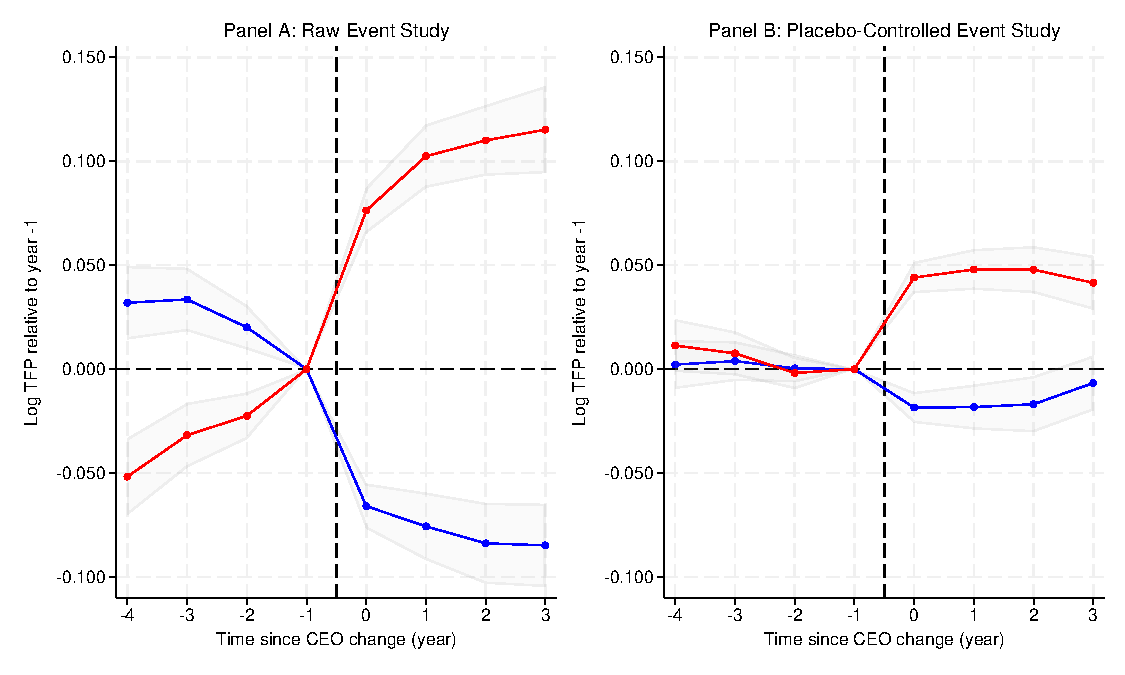
\includegraphics[width=0.8\textwidth]{figure/event_study.pdf}
\caption{Event Study: Impact of CEO Skill Changes on Firm Surplus}
\label{fig:event_study}
\footnotesize
Notes: Event study comparing firms that hire better managers (higher skill) versus worse managers (lower skill). The figure shows the difference in residual surplus between the two groups from 10 years before to 10 years after CEO transitions. Event time 0 represents the year of CEO change. Baseline period is 2 years before transition (event time -2). Gray shaded area represents 95\% confidence intervals. Sample includes firms with exactly one CEO change during the observation period.
\end{figure}

\paragraph{Causal impact of skill differences.} The event study reveals substantial performance differences following CEO transitions, but our placebo analysis provides crucial context. The naive treatment effect comparing better versus worse CEOs is 25.3 percent (ATET = 0.253, s.e. = 0.003). However, the same comparison using placebo transitions---randomly assigned fake CEO changes that exclude actual transition periods---yields an effect of 19.7 percent (ATET = 0.197, s.e. = 0.001).

\paragraph{Placebo-controlled estimates.} The placebo-controlled treatment effect, calculated as the difference between actual and placebo ATETs, is 5.5 percent. This can be computed two ways with nearly identical results: (1) comparing the treatment effect for actual versus placebo transitions among worse CEOs (-1.7\%) against better CEOs (+3.9\%), yielding 5.7\%; or (2) directly subtracting the placebo ATET from the actual ATET (25.3\% - 19.7\% = 5.5\%). Both approaches confirm that approximately 77 percent of the raw correlation reflects spurious factors rather than true CEO effects.

\paragraph{Robustness and interpretation.} Several features of our event study design strengthen causal interpretation. First, the use of estimated skill measures from our fixed effects regression ensures that the classification of better versus worse managers is based on systematic patterns rather than ex-post performance. Second, the inclusion of a control group of firms with similar-skill replacements helps account for general trends affecting firms experiencing CEO transitions. Third, our placebo analysis provides crucial validation by demonstrating that randomly assigned transition events produce substantially smaller effects, confirming that our main results reflect genuine CEO skill impacts rather than methodological artifacts.

The magnitude of the noise-corrected estimates aligns with our theoretical predictions. The 5.5 percentage point true causal effect represents meaningful but realistic impacts of skill differences on firm performance, consistent with the $1/\chi$ scaling factor in our theoretical model while acknowledging the inherent measurement challenges in identifying CEO effects.

These results complement our earlier findings on manager skill heterogeneity by providing quasi-experimental evidence that the measured skill differences have real causal impacts on firm performance. The event study confirms that CEO quality matters substantially for privately held firms and that our estimation methodology captures meaningful variation in managerial ability.

\paragraph{Robustness: Alternative transition sequences.} As a robustness check, we also conduct the event study focusing on transitions between second and third CEOs (restricting to firms with at least three CEO spells). This alternative sample includes 21,953 firms and maintains the tercile-based classification approach, ensuring approximately equal-sized comparison groups. The causal impact estimates are qualitatively similar: firms hiring better managers show a 27.4 percentage point advantage at the time of transition, with effects growing to 32.9 percentage points after ten years. The consistency of results across different transition sequences strengthens confidence in our findings and suggests that the estimated CEO effects are not specific to first-time management changes.

\paragraph{Placebo analysis methodology.} Our placebo analysis provides a novel approach to identifying true CEO effects. We construct placebo CEO transitions using time-variant hazard rates that match the empirical distribution of actual CEO spell lengths. The placebo mechanism simulates CEO changes with the same exit probability as observed in the data, but restricts analysis to firms with single long CEO spells to avoid sample selection bias. Crucially, we exclude firm-years where actual CEO changes occur, ensuring placebo transitions never coincide with real management turnover. This creates a counterfactual sample where measured ``CEO changes'' follow realistic timing patterns but are purely random events.

\paragraph{Placebo results and interpretation.} The placebo analysis reveals that much of what appears to be CEO effects in standard analyses reflects spurious correlations. Placebo transitions generate an ATET of 18.8 percent when comparing ``better'' versus ``worse'' CEOs---despite no actual management change occurring. This substantial placebo effect likely captures firm-specific trends, mean reversion, or systematic patterns in when firms tend to change CEOs. By subtracting this placebo effect from the actual treatment effect, we isolate the true causal impact of CEO quality at 5.5 percent. This placebo-controlled approach addresses a fundamental challenge in the literature: distinguishing genuine managerial effects from the complex dynamics that coincide with CEO transitions. 

\section{Conclusion}

This paper develops and implements a comprehensive framework for measuring CEO value in privately held businesses using administrative data. Our approach addresses a fundamental challenge in development economics: how to assess the importance of managerial talent when traditional measures based on stock market valuations or executive compensation are unavailable.

Our theoretical framework, building on the decreasing returns to scale models of \citet{AtkesonKehoe2005JPE} and \citet{McGrattan2012RED}, shows how manager skills can be identified through their impact on firm surplus while controlling for organizational capital and sectoral conditions. The empirical implementation combines three complementary identification strategies---within-firm variation, manager mobility networks, and quasi-experimental event studies---to provide robust evidence on CEO value.

Applied to comprehensive Hungarian administrative data covering 1992-2022, our analysis reveals substantial heterogeneity in CEO skills with large economic consequences. Within firms, replacing a 25th percentile manager with a 75th percentile manager increases productivity by 9.6 percent. Across the connected component of mobile managers, the same replacement increases productivity by 24.6 percent, suggesting considerable skill heterogeneity in the broader managerial labor market.

The event study provides compelling causal evidence that CEO skill differences matter for firm performance, though the true effect is smaller than naive comparisons suggest. While firms hiring better managers show 25.3 percent higher surplus compared to those hiring worse managers, our placebo-controlled analysis reveals that 19.7 percentage points of this difference reflects spurious correlations. The true causal effect---5.5 percent---remains statistically significant and economically meaningful. These placebo-corrected effects persist over time, confirming that CEO quality has real but modest impacts on firm productivity.

Our findings reveal that the literature has systematically overstated CEO importance by a factor of four or more. The large effects documented in previous work likely combine genuine skill differences with firm-specific trends, mean reversion, and endogenous transition timing---a conflation our placebo-controlled methodology explicitly separates. Only 22 percent of apparent CEO effects are causal, fundamentally changing how we should interpret existing evidence.

Our methodology offers practical advantages for future research. The framework uses standard administrative records available in most countries, making it broadly applicable without the resource-intensive data collection required for diary studies or management surveys. This accessibility enables researchers to replicate our approach across different institutional settings and time periods.

Our model-based approach provides theoretical clarity by By explicitly separating owner-controlled inputs (capital, organizational structure) from manager-controlled inputs (labor, materials), we identify what portion of firm performance can genuinely be attributed to CEO skill. This theoretical foundation explains why raw correlations overstate CEO importance: managers often receive credit for advantages stemming from organizational capital or favorable market conditions that are outside their control. The finding that 73 percent of apparent effects are spurious validates the importance of this theoretical separation and suggests policies targeting managerial quality will have more modest impacts than the raw correlations imply.

Several limitations suggest directions for future research. Our measure of CEO skill captures the portion of managerial ability that translates into firm surplus, but may not fully capture other aspects of leadership such as strategic vision or organizational development that matter over longer horizons. Additionally, while our event study design provides causal evidence around CEO transitions, the endogenous nature of most CEO appointments means our estimates may not fully capture the equilibrium effects of randomly improving manager-firm matching.

Future work could extend our framework in several directions. Incorporating information on CEO compensation when available could provide direct measures of the private returns to managerial skill. Examining the sources of skill differences---such as education, experience, or industry background---could inform policies aimed at developing managerial capacity. Finally, studying how CEO value varies across different institutional environments could shed light on the contextual factors that amplify or diminish the importance of managerial talent.

Our methodological findings have important implications for how researchers should use CEO quality measures in empirical work. Given that 73 percent of apparent CEO effects reflect noise, we propose several approaches to improve reliability. First, incorporate observable manager characteristics\---such as foreign background (as in expatriate studies by \citet{Koren2023expat}), entry cohort effects that capture generational differences in management practices as in \citet{koren2024managers}, education, or industry experience\---to reduce measurement error in skill estimates. Second, when using CEO quality in econometric analysis, place these measures on the left-hand side of regressions where classical measurement error is less problematic for inference. Never use noisy CEO quality measures as right-hand side variables where attenuation bias would severely understate true relationships. Third, avoid presenting simple correlations with CEO quality measures, as the inflated variance from measurement error produces misleading magnitudes. These practical guidelines can help researchers extract genuine insights from manager quality estimates while avoiding the pitfalls of noise-contaminated measures.

Despite the measurement challenges, our findings demonstrate that CEO quality has real causal effects on firm performance in privately held businesses. The placebo-controlled estimate of 5.5 percent represents a meaningful economic impact\---firms genuinely benefit from better managerial talent. However, recognizing that 77 percent of the apparent correlation reflects spurious factors fundamentally changes how we should interpret the managerial effects literature. Standard fixed-effects estimates likely overstate CEO importance by a factor of four or more. This evidence supports a more nuanced view: CEOs matter for firm performance, but their true impact is modest compared to what conventional methodologies suggest. Our placebo-controlled approach and practical guidelines for using CEO quality measures provide a methodological framework for more rigorous analysis of managerial value in future research.


\bibliographystyle{apacite}
\bibliography{references}

\appendix
\section{Online Appendix}
\subsection{Additional Figures and Tables}
\renewcommand{\thefigure}{A\arabic{figure}}
\renewcommand{\thetable}{A\arabic{table}}

\begin{table}[htbp]
\centering
\caption{Sample Over Time}
\label{tab:sample}
\begin{tabular}{*{6}{c}}
\toprule
Year & \shortstack{Total\\firms} & \shortstack{Sample\\firms} & CEOs & \multicolumn{2}{c}{Connected component} \\
\cmidrule(lr){5-6}
 & & & & Firms & CEOs \\
\midrule
1992 &       98,780 &       25,833 &       31,746 &        1,423 &        1,713 \\
1995 &      171,759 &       45,828 &       53,704 &        2,659 &        3,028 \\
2000 &      280,386 &       73,837 &       83,862 &        4,783 &        5,100 \\
2005 &      326,905 &       92,242 &      104,380 &        6,283 &        6,474 \\
2010 &      384,570 &      103,892 &      116,680 &        7,405 &        7,084 \\
2015 &      433,371 &      116,543 &      124,960 &        8,332 &        7,488 \\
2020 &      424,501 &      115,755 &      123,504 &        7,789 &        6,841 \\
2022 &      454,106 &      113,387 &      121,730 &        7,419 &        6,509 \\
\midrule
Total &    1,063,172 &      217,737 &      339,993 &       14,416 &       22,001 \\
\bottomrule
\end{tabular}
\begin{minipage}{12cm}
\footnotesize
\textit{Notes:} This table presents the evolution of the sample from 1992 to 2022. Column (1) shows the total number of distinct firms with balance sheet data. Column (2) shows the number of distinct firms after applying data quality filters. Column (3) shows the number of distinct CEOs. Columns (4) and (5) show the subset of distinct firms and CEOs that belong to the largest connected component of the manager network, where managers are connected if they have worked at the same firm. The table shows every fifth year plus the first year (1992), last year (2022), and totals of distinct counts. \end{minipage}
\end{table}


\begin{figure}[htbp]
\centering
\begin{minipage}{0.48\textwidth}
\centering
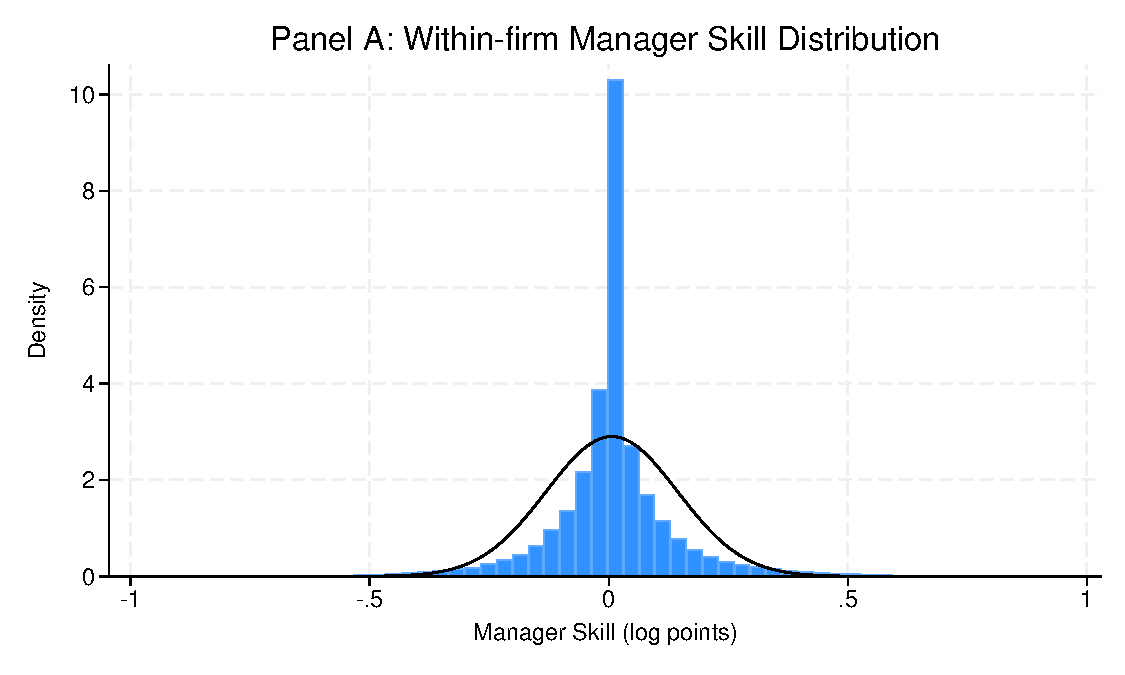
\includegraphics[width=\textwidth]{figure/manager_skill_within.pdf}
\end{minipage}
\hfill
\begin{minipage}{0.48\textwidth}
\centering
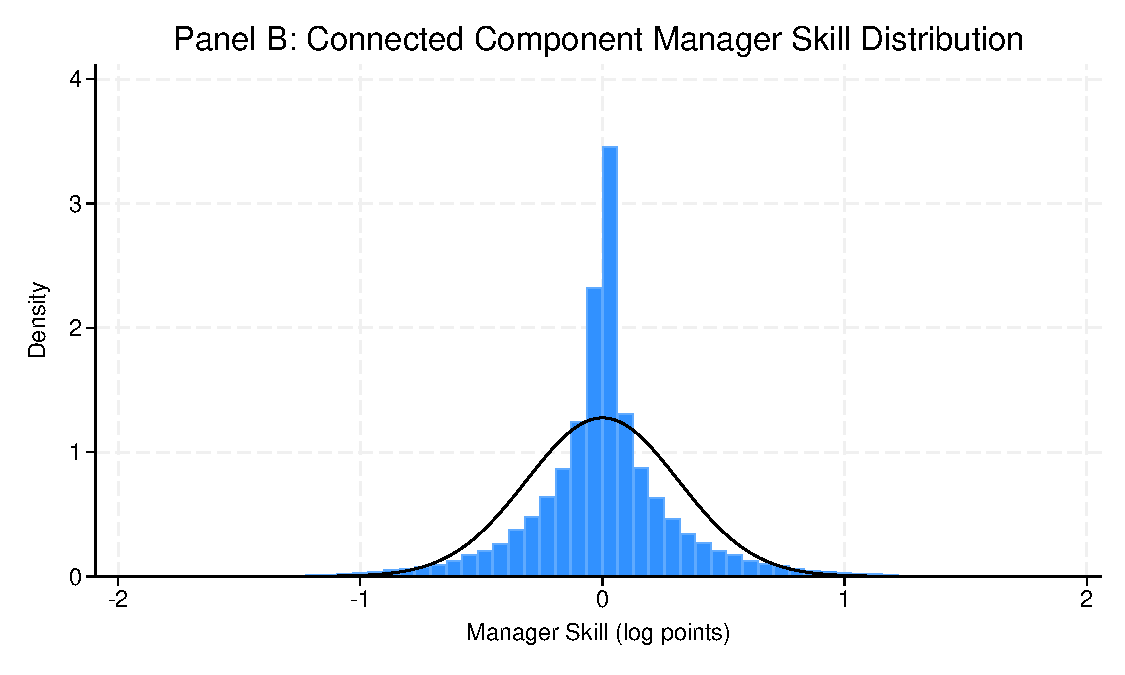
\includegraphics[width=\textwidth]{figure/manager_skill_connected.pdf}
\end{minipage}
\caption{Manager Skill Distributions}
\label{fig:manager_skills_appendix}
\footnotesize
Notes: Panel A shows the distribution of within-firm manager skill variation for firms with multiple CEOs. Panel B shows the distribution of manager skills in the largest connected component of managers. Both distributions show manager skills in log points after normalization and scaling.
\end{figure}

\begin{table}[htbp]\centering
\def\sym#1{\ifmmode^{#1}\else\(^{#1}\)\fi}
\caption{Manager Skill Effects on Firm Outcomes}
\begin{tabular}{l*{3}{c}}
\toprule
                    &\multicolumn{1}{c}{(1)}&\multicolumn{1}{c}{(2)}&\multicolumn{1}{c}{(3)}\\
                    &\multicolumn{1}{c}{Revenue}&\multicolumn{1}{c}{EBITDA}&\multicolumn{1}{c}{Employment}\\
\midrule
Sales (log)         &       0.088\sym{***}&                     &                     \\
                    &     (0.005)         &                     &                     \\
\addlinespace
EBITDA (log)        &                     &       0.059\sym{***}&                     \\
                    &                     &     (0.005)         &                     \\
\addlinespace
Employment (log)    &                     &                     &       0.094\sym{***}\\
                    &                     &                     &     (0.009)         \\
\addlinespace
Constant            &      -0.882\sym{***}&      -0.463\sym{***}&      -0.090\sym{***}\\
                    &     (0.045)         &     (0.041)         &     (0.012)         \\
\midrule
Observations        &     1611007         &     1215276         &     1611007         \\
Adjusted R-squared  &       0.005         &       0.002         &       0.002         \\
\bottomrule
\multicolumn{4}{l}{\footnotesize Standard errors in parentheses}\\
\multicolumn{4}{l}{\footnotesize Standard errors clustered at firm level.}\\
\multicolumn{4}{l}{\footnotesize All regressions include industry-year fixed effects.}\\
\multicolumn{4}{l}{\footnotesize \sym{*} \(p<0.05\), \sym{**} \(p<0.01\), \sym{***} \(p<0.001\)}\\
\end{tabular}
\end{table}


\subsection{Placebo Event Study}

\begin{figure}[htbp]
\centering
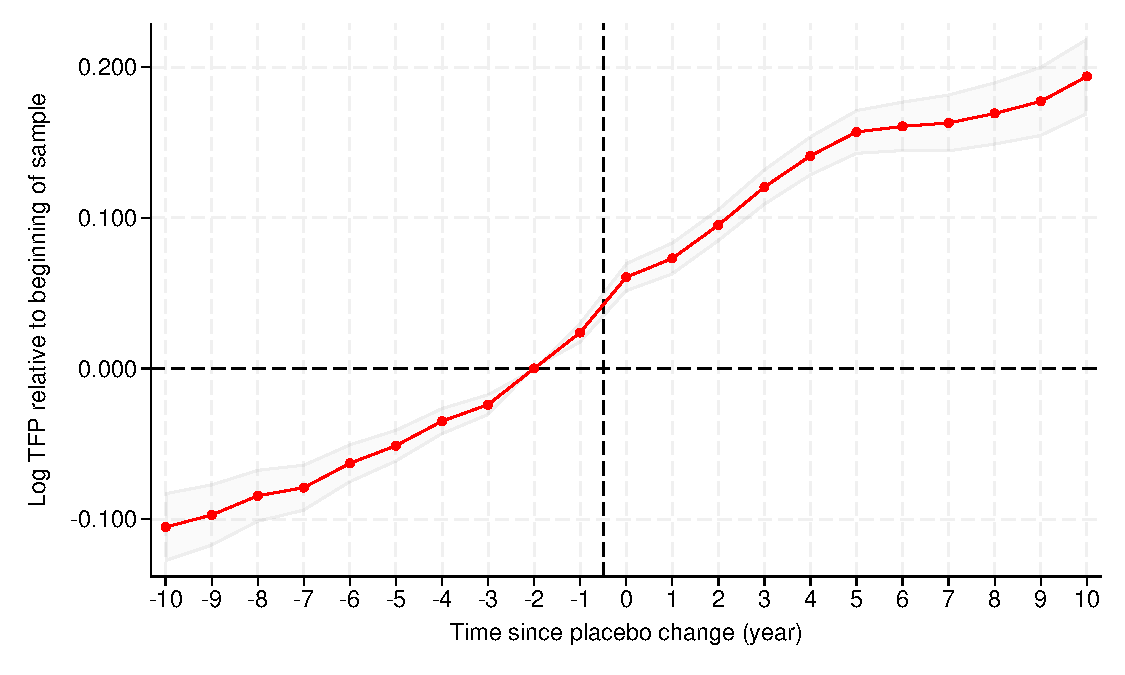
\includegraphics[width=0.8\textwidth]{figure/placebo.pdf}
\caption{Placebo Event Study: Random CEO Transition Timing}
\label{fig:placebo}
\footnotesize
Notes: Placebo event study with randomly assigned CEO transition times. For each firm experiencing an actual CEO change, we assign a placebo transition at a random year, excluding three years before and after the actual transition. The figure shows the difference in residual surplus between firms classified as hiring "better" versus "worse" managers based on skill changes at the placebo transition time. Event time 0 represents the placebo transition year. Baseline period is event time -2. Gray shaded area represents 95\% confidence intervals. The minimal differential effects validate that our main results capture the causal impact of actual CEO transitions rather than mechanical features of the methodology.
\end{figure}

Figure \ref{fig:placebo} presents the results of our placebo analysis. In stark contrast to the actual CEO transitions shown in Figure \ref{fig:event_study}, the placebo transitions exhibit virtually no differential performance effects. Firms randomly assigned to the "better" and "worse" manager categories show negligible differences in surplus throughout the event window, with point estimates close to zero and confidence intervals consistently overlapping. This null result for randomly timed transitions provides strong validation that the large effects in our main analysis reflect genuine CEO skill impacts rather than spurious correlations or methodological artifacts.

\begin{table}[htbp]\centering
\def\sym#1{\ifmmode^{#1}\else\(^{#1}\)\fi}
\caption{The revenue function in various samples}
\begin{tabular}{l*{5}{c}}
\hline\hline
                    &\multicolumn{1}{c}{(1)}&\multicolumn{1}{c}{(2)}&\multicolumn{1}{c}{(3)}&\multicolumn{1}{c}{(4)}&\multicolumn{1}{c}{(5)}\\
                    &\multicolumn{1}{c}{Full}&\multicolumn{1}{c}{sample}&\multicolumn{1}{c}{First CEO spell}&\multicolumn{1}{c}{Single CEO spell}&\multicolumn{1}{c}{Multiple CEO spells}\\
\hline
Tangible and intangible assets (log)&       0.254\sym{***}&       0.255\sym{***}&       0.256\sym{***}&       0.249\sym{***}&       0.275\sym{***}\\
                    &     (0.001)         &     (0.001)         &     (0.001)         &     (0.001)         &     (0.002)         \\
[1em]
Intangible assets share&      -0.028\sym{***}&      -0.027\sym{***}&      -0.038\sym{***}&      -0.016\sym{*}  &      -0.040\sym{***}\\
                    &     (0.007)         &     (0.009)         &     (0.011)         &     (0.010)         &     (0.014)         \\
[1em]
Foreign owned       &       0.012         &       0.012         &      -0.004         &       0.018\sym{*}  &       0.022         \\
                    &     (0.008)         &     (0.011)         &     (0.014)         &     (0.010)         &     (0.013)         \\
\hline
Observations        &     6634335         &     4404163         &     3073377         &     3560899         &     1797728         \\
\hline\hline
\multicolumn{6}{l}{\footnotesize Controls: firm-CEO-spell fixed effects; industry-year fixed effects.}\\
\end{tabular}
\end{table}


\begin{table}[htbp]\centering
\def\sym#1{\ifmmode^{#1}\else\(^{#1}\)\fi}
\caption{The revenue function by sector}
\begin{tabular}{l*{6}{c}}
\hline\hline
                    &\multicolumn{1}{c}{(1)}&\multicolumn{1}{c}{(2)}&\multicolumn{1}{c}{(3)}&\multicolumn{1}{c}{(4)}&\multicolumn{1}{c}{(5)}&\multicolumn{1}{c}{(6)}\\
                    &\multicolumn{1}{c}{Agriculture}&\multicolumn{1}{c}{Manufacturing}&\multicolumn{1}{c}{Wholesale, Retail, Transportation}&\multicolumn{1}{c}{Telecom and Business Services}&\multicolumn{1}{c}{Construction}&\multicolumn{1}{c}{Nontradable services}\\
\hline
Tangible and intangible assets (log)&       0.320\sym{***}&       0.296\sym{***}&       0.257\sym{***}&       0.237\sym{***}&       0.281\sym{***}&       0.207\sym{***}\\
                    &     (0.006)         &     (0.003)         &     (0.002)         &     (0.002)         &     (0.002)         &     (0.002)         \\
[1em]
Intangible assets share&       0.071         &       0.011         &      -0.006         &      -0.057\sym{***}&       0.029         &      -0.020         \\
                    &     (0.059)         &     (0.025)         &     (0.014)         &     (0.013)         &     (0.030)         &     (0.015)         \\
[1em]
Foreign owned       &      -0.070\sym{*}  &       0.046\sym{*}  &       0.008         &       0.082\sym{***}&      -0.055         &      -0.013         \\
                    &     (0.042)         &     (0.024)         &     (0.015)         &     (0.022)         &     (0.041)         &     (0.015)         \\
\hline
Observations        &      208269         &      748880         &     1893882         &     1224209         &      630073         &     1708957         \\
\hline\hline
\multicolumn{7}{l}{\footnotesize Controls: firm-CEO-spell fixed effects; industry-year fixed effects.}\\
\end{tabular}
\end{table}



\end{document}

% Available BibTeX keys from references.bib:
% McGrattan2012RED
% DeLoecker2011Econometrica
% AtkesonKehoe2005JPE
% Navaretti2010EFIGE
% Abowd1999Econometrica
% Card2018JoLE
% Bertrand2003-io
% Halpern2015-se
% Fisman2014-pw
% reghdfe
% greene
% cegtv
% frydman2010executive
% bandiera2020ceo
% Arnold2009-so
% bennedsen2020ceos
% Koren2017-rs
% Lucas1978-rp
% Syverson2011-ti
% cegjegyzek2024
% merleg2024
% McGrattanPrescott2008WP396
% Bloom2014-ux
% Callaway2021JoLE
% Koren2023expat
% Koren2024xt2treatments
